%------------------------ Packages ------------------------
\documentclass[12pt,a4paper]{article}
\usepackage[latin1]{inputenc}
\usepackage[T1]{fontenc}
\usepackage[pdftex]{graphicx}
\usepackage{float}
\usepackage{amsmath}
\usepackage{amssymb}
\usepackage[FIGTOPCAP]{subfigure}
\usepackage{color}
\usepackage[hidelinks]{hyperref}

\newcommand{\version}{\IfFileExists{../../version.txt}
{\input{../../version.txt}}
{\input{../../../version.txt}}
}

\newcommand{\command}[1]{%
\indent \fcolorbox{black}{white}{%
   \begin{minipage}{\dimexpr\textwidth-\parindent\relax}%
      #1
   \end{minipage}%
}
}

\newsavebox{\FVerbBox}
\newenvironment{sample}
{\par \vspace{0.2cm} \begin{lrbox}{\FVerbBox}
\begin{minipage}{\dimexpr\textwidth-\parindent\relax}}
{\end{minipage}
\end{lrbox}
\fcolorbox{black}{lightgray}{\usebox{\FVerbBox}}
\vspace{0.2cm}}

\newenvironment{sampletitle}
{\vspace{0.2cm} \noindent\textbf{Example} :
\begin{sample}}
{\end{sample}}

\newcommand{\samplecomment}[1]{%

\textit{#1}
}

\newcommand{\seealso}[1]{\vspace{0.2cm} \noindent\textbf{See also} :\par #1}

% tikz
\usetikzlibrary{calc}
\usetikzlibrary{arrows}
\usetikzlibrary{shadows}

\tikzset{block/.style={draw, text centered, fill=gray!10,drop shadow}}
\tikzset{connect/.style={draw, line width=1 pt}}

\begin{document}

\begin{center}
\textbf{\huge  \underline{Negation operator}}
\end{center}
\vspace{0.5cm}

The negation operator is a basic operation used to replace a greyscale or a binary image by its negative image. 
At each point in the image, the new value is the pixel complement on IN\_SIZE bits.
\\


\begin{figure}[h!]
\centering
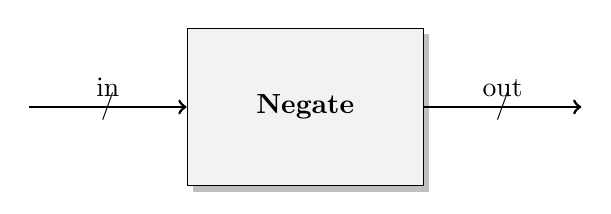
\begin{tikzpicture}
\node[block,rectangle,minimum height=2cm,minimum width=3cm] (bloc) {\textbf{Negate}};

\path[connect,<-] ([yshift=0.0cm]bloc.west) -- node{/} node[above]{in} ++(-2cm,0);

\path[connect,->] ([yshift=0.0cm]bloc.east) -- node{/} node[above]{out} ++(2cm,0);
 ([xshift=0.5cm,yshift=-0.6cm]bloc.north);

\end{tikzpicture}
\end{figure}

\vspace{0.5cm}

%\begin{figure}[!h]
%\centering
%\subfigure[Initial greyscale image]{
%
\includegraphics[width=5cm]{greyscale.png}}
%\hspace{2cm}
%\subfigure[Negated image]{
%\includegraphics[width=5cm]{negate1.png}}
%\vspace{2cm}
%\subfigure[Initial binary image]{
%
\includegraphics[width=5cm]{binary.png}}
%\hspace{2cm}
%\subfigure[Negated binary image]{
%\includegraphics[width=5cm]{negate2.png}}
%\end{figure}

\section*{Properties}
\properties{
enable           & bool & Enable the processing \\ 
}

\vspace{0.5cm}

\section*{Constants}

\constants{
CLK\_PROC\_FREQ & Frequency clock of the process \\
IN\_SIZE & Size of the input flow : 1 byte (greyscale image) or 1 bit (binary image)\\
OUT\_SIZE & Size of the output flow : 1 byte (greyscale image) or 1 bit (binary image)\\
}



\section*{Equivalence}
\subsection*{Matlab}

\lstset{language=Matlab}
\begin{lstlisting}
I; % image matrix
I_negated = imcomplement(I);
% This functions takes a grayscale or a binary image

\end{lstlisting}

\url{https://fr.mathworks.com/help/images/ref/imcomplement.html}



\section*{Mathematical formalism}

For each pixel $nPx$ of the original image, the following operation is applied:


\centering

$\displaystyle nPx $ 	$\textstyle =$ 	$\displaystyle \bar{Px}$

\vspace{0.5cm}



\end{document}